\chapter{中值定理及导数的应用}

\makepart{单项选择题}

\begin{problem}
若 $f(x)$ 在 $(a,b)$ 内单调增加, 则必有\pickin{D}.
\begin{abcd} 	
	\item $f'\left( x \right) < 0;$
	
	\item $f'\left( x \right) > 0$
	
	\item $f'\left( x \right) \geq 0;$
	
	\item A, B, C 都不对.
\end{abcd}

\kpoint{函数单调性的判别法}
\end{problem}

\begin{problem}
函数 $y = f\left( x \right)$ 满足条件:
$f\left( 0 \right) = 1,f'\left( 0 \right) = 0,$ 当 $x \neq 0$ 时,
$f'\left( x \right) > 0,$ $f''\left( x \right)\left\{ \begin{matrix}
\ < 0\ ,\ \ \ x < 0 \\
\ > 0\ ,\ \ \ x > 0 \\
\end{matrix}\ , \right.\ $ 它的图形是\pickin{B}.

%	\begin{figure}
%		\centering
%		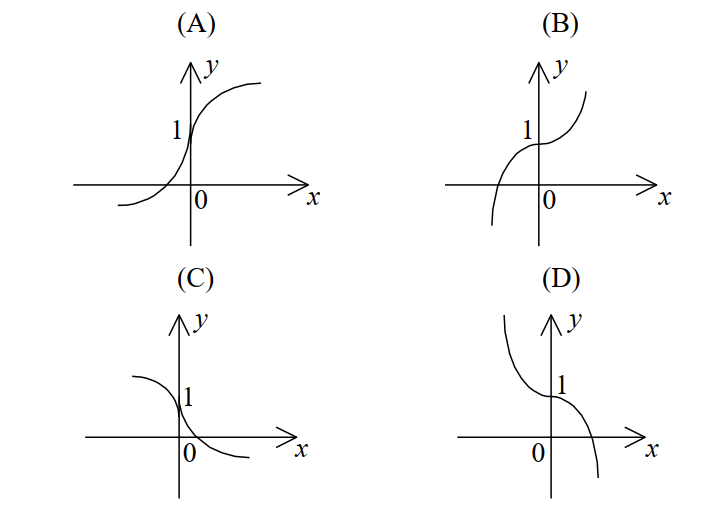
\includegraphics{D:/sslchi.github.io/calculus/HW_chap4a.png}
%		\caption{HW\_chap1a}
%	\end{figure}


\kpoint{曲线的凸凹性与拐点}
\end{problem}
\begin{problem}
设 $\displaystyle f\left( x \right) = \frac{\ln x}{x}$, 则使不等式
$\displaystyle \frac{\ln a}{a} > \frac{\ln b}{b}$ 成立的条件是\pickin{B}.

\begin{abcd} 
	
	\item $\ 0 < a < b;$
	
	\item $\e < a < b;$
	
	\item $\ 0 < b < a;$
	
	\item $\e < b < a.$

\end{abcd}

\kpoint{函数单调性的判别法}
\end{problem}

\begin{problem}
关于函数 $y = x - \ln x$ 的极值, 结论正确的是\pickin{A}.

\begin{abcd} 
\item 有极小值 $1$;

\item 有极大值 $1$;

\item 无极值 $\e - 1$;

\item 有极小值 $\e - 1$.

\end{abcd}

\kpoint{函数极值的第一充分条件}
\end{problem}

\begin{problem}
关于函数 $y = 2x - {\ln\left( 4x \right)}^{2}$ 的极值,
结论正确的是\pickin{B}.

\begin{abcd} \item 有极大值 $2 - 4\ln 2;$

\item 有极小值 $2 - 4\ln 2;$

\item 无极值;

\item 有极小值 $\frac{1}{2}.$

\end{abcd}


\kpoint{函数极值的第一充分条件}
\end{problem}

\begin{problem}
曲线 $y = 3x^{2} - x^{3}$ 在\pickin{B}

\begin{abcd} 
\item $\left( 1, + \infty \right)$是凹的, $\left( - \infty,1 \right)$
是凸的;

\item $\left( 1, + \infty \right)$是凸的, $\left( - \infty,1 \right)$
是凹的;

\item $\left( 0, + \infty \right)$内是凸的,
在$\left( - \infty,0 \right)$是上凹的;

\item $\left( 0, + \infty \right)$ 内是上凹的,
$\left( - \infty,0 \right)$ 是上凸的;

\end{abcd} 

\kpoint{曲线的凸凹性判别}
\end{problem}

\begin{problem}
曲线 $y = x^{2}\ln x$ 在点
$\displaystyle \left( \frac{1}{\e^{4}},\frac{1}{\e^{2}} \right)$ 近邻是\pickin{A}.

\begin{abcd} \item 向上凸的; \item 向上凹的;

\item 左侧近邻向上凸, 右侧近邻向上凹;

\item 左侧近邻向上凹, 右侧的邻向上凸;

\end{abcd}

\kpoint{曲线的凸凹性判别}
\end{problem}

\begin{problem}
曲线 $y = \e^{- x^{2}}$ 的拐点情况是\pickin{C}.

\begin{abcd} \item 没有拐点;

\item 有一个拐点;

\item 有两个拐点;

\item 有三个拐点.

\end{abcd}

\kpoint{曲线的凸凹性与拐点}

\end{problem}

\begin{problem}
若 $\left( x_{0},f\left( x_{0} \right) \right)$ 为连续曲线
$y = f\left( x \right)$ 上的凹弧与凸弧分界点, 则\pickin{A}.

\begin{abcd} \item $\left( x_{0},f\left( x_{0} \right) \right)$ 必为曲线的拐点;

\item $\left( x_{0},f\left( x_{0} \right) \right)$ 必定为曲线的驻点;

\item $x_{0}$ 为 $f\left( x \right)$ 的极值点;

\item $x_{0}$ 必定不是 $f\left( x \right)$ 的极值点;

\end{abcd}

\kpoint{曲线的凸凹性与拐点}
\end{problem}


\begin{problem}
曲线 $\left\{ \begin{matrix}
 x = a(t - \sin t) \\
 y = a(1 - \cos t) \\
\end{matrix}(a > 0) \right.\ $\pickin{C}.

\begin{abcd} \item 有无穷多个拐点;

\item 有两个拐点;

\item 无拐点;

\item 有一个拐点.

\end{abcd}

\kpoint{曲线的凸凹性与拐点}
\end{problem}


\begin{problem} 
点 $(0,1)$ 是曲线 $y = ax^{3} + bx^{2} + c$ 的拐点, 则必有\pickin{B}.

\begin{abcd} \item $a = 1,\ b = - 3,\ c = 1;$

\item $a$ 任意, $b = 0,\ c = 1;$

\item $a = 1,\ b = 0,$ $c$ 任意;

\item $b = - 3a$, $a$ 任意, $c = 1$.

\end{abcd}

\kpoint{曲线的凸凹性与拐点}
\end{problem}

\begin{problem}
关于曲线 $y = \ln x$ 的渐近线, 下述结论正确的是\pickin{B}.

\begin{abcd} \item 只有水平渐近线;

\item 只有铅直渐近线;

\item 既有水平渐近线, 又有铅直渐近线 ;

\item 既没有水平渐近线, 也没有铅直渐近线.

\end{abcd}

\kpoint{曲线的渐近线}
\end{problem}

\begin{problem}
$\displaystyle \lim\limits_{x \rightarrow \frac{\pi}{2}}\left( \frac{\cos 5x}{\cos 3x} \right)$=
\pickin{A}

\begin{abcd} \item $- 5/3;$

\item $- 1;$

\item $1;$

\item $5/3.$

\end{abcd}

\kpoint{洛必达法则}
\end{problem}

\begin{problem}
在区间 $\lbrack 0,8\rbrack$ 内, 对函数
$f\left( x \right) = \sqrt[3]{8x - x^{2}}$, 罗尔定理\pickin{C}.

\begin{abcd} \item 不成立;

\item 成立, 并且 $f'\left( 2 \right) = 0;$

\item 成立, 并且 $f'\left( 4 \right) = 0;$

\item 成立, 并且 $f'\left( 8 \right) = 0$.

\end{abcd}

\kpoint{罗尔定理}
\end{problem}

\begin{problem}
设 $f(x)\ $ 在 $\left\lbrack a,b \right\rbrack$ 上连续, 在
$\left( a,b \right)$ 内可导, 记(I)
$f\left( a \right) = f\left( b \right)$; (II) 在 $\left( a,b \right)$
内至少存在 $\xi$, 使 $f'\left( \xi \right) = 0$, 则\pickin{A}.

\begin{abcd} \item(I)是(II) 的充分但非必要条件;

\item(I)是(II) 的必要但非充分条件;

\item (I) 是(II) 的充要条件;

\item (I) 是(II) 既非充分, 也非必要条件.

\end{abcd}

\kpoint{罗尔定理}
\end{problem}

\begin{problem}
设 $f(x) = \left\{ \begin{matrix}
3 - x^{2},\ \ \ \ 0 \leq |x| \leq 1 \\
\displaystyle \frac{2}{x},\ \ \ \ 1 < |x| \leq 2 \\
\end{matrix}\ \ , \right.\ $ 则在区间内 $(0,2)$ 满足
$f\left( 2 \right) - f\left( 0 \right) = f'\left( \xi \right)\left( 2 - 0 \right)$
的 $\xi$ 值\pickin{C}.

\begin{abcd} \item 只有一个;

\item 不存在;

\item 有两个;

\item 有三个.

\end{abcd}

\kpoint{拉格朗日中值定理}
\end{problem}

\begin{problem}
设 $a < b,ab < 0,f\left( x \right) =\displaystyle  \frac{1}{x}$, 则在
$a < x < b$ 内使
$f\left( b \right) - f\left( a \right) = f'\left( \xi \right)\left( b - a \right)$
成立的点 $\xi$ \pickin{C}.

\begin{abcd} \item 只有一点;

\item 有两点;

\item 不存在;

\item 是否存在,与 $a,b\ $ 的具体数值有关.

\end{abcd}

\kpoint{拉格朗日中值定理}
\end{problem}

\begin{problem}
设 $f(x)$ 有直至 $n + 1$ 阶导数, 则
$\displaystyle f\left( x \right) = \sum_{k = 1}^{n}{\frac{f^{\left( k \right)}\left( 0 \right)}{k!}x^{k}} + R_{n}\left( x \right)$式中拉格朗日型余项
$R_{n}\left( x \right)$ =\pickin{B}(设 $0 < \theta < 1$)

\begin{abcd} \item $\displaystyle \frac{f^{\left( n \right)}\left( \theta x \right)}{n!}x^{n};$

\item
$\displaystyle \frac{f^{\left( n + 1 \right)}\left( \theta x \right)}{\left( n + 1 \right)!}x^{n + 1};$

\item
$\displaystyle \frac{f^{\left( n + 1 \right)}\left( x \right)}{\left( n + 1 \right)!}\left( \theta x \right)^{n + 1};$

\item
$\displaystyle \frac{f^{\left( n + 1 \right)}\left( \theta \right)}{\left( n + 1 \right)!}x^{n + 1}$.

\end{abcd}

\kpoint{泰勒公式(大纲无此内容)}
\end{problem}

\begin{problem}
已知函数 $f\left( x \right) = x^{3} + ax^{2} + bx$ 在点 $x = 1$
处取得极值 $- 2$, 则\pickin{B}.

\begin{abcd}

\item $a = - 3,\ b = 0$ 且点 $\ x = 1\ $为函数 $f(x)$ 的极小值;

\item $a = 0,\ b = - 3$ 且点 $x = 1$ 为函数 $f(x)$ 的极小值;

\item $a = - 3,\ b = 0$ 且点 $x = 1$ 为函数 $f(x)$ 的极大值;

\item $a = 0,\ b = - 3\ $ 且点 $x = 1\ $为函数 $f(x)$ 的极大值.

\end{abcd}

\kpoint{函数极值的第一充分条件}
\end{problem}

\begin{problem} 
函数
$f\left( x \right) = \displaystyle \frac{\sqrt{x - 1}}{x\left( x - 1 \right)\left( x - 2 \right)}$
的所有渐近线有\pickin{B}条

\begin{abcd} \item $4;$

\item $3;$

\item $2;$

\item $1$.

\end{abcd}

\kpoint{曲线的渐近线}
\end{problem}

\makepart{填空题}

\begin{problem} 曲线 $y = 1 - \sqrt[3]{x - 2}$ 的拐点是\fillin{$(2,1)$}.

\kpoint{曲线的凸凹性与拐点}
\end{problem}

\begin{problem} 设函数 $f(x)$ 在 $(a,b)$ 内可导且满足
$f'\left( x \right) \equiv 0$, 则在 $(a,b)$ 内 $f(x)\ $=
\fillin{ $C,\ C$ 为常数}.

\kpoint{拉格朗日中值定理}
\end{problem}

\begin{problem} 设函数 $f(x)$ 在 $x = 0$ 处具有二阶导数, 且 $f(0) = 0,$
$f'\left( 0 \right) = 1,$ $f''\left( 0 \right) = 3,$ 则极限
$\displaystyle \lim\limits_{x \rightarrow 0}\frac{f\left( x \right) - x}{x^{2}}$ =\fillin{ $\displaystyle \frac{3}{2}$}.

\kpoint{洛必达法则}
\end{problem}

\begin{problem} $\displaystyle \lim\limits_{x \rightarrow 0}\frac{\ln{\cos a}x}{\ln{\cos b}x}$
的值等于\fillin{$\displaystyle \frac{a^{2}}{b^{2}}.$}, $\left( b \neq 0 \right).$.



\kpoint{洛必达法则}
\end{problem}


\begin{problem} 设 $a > 0,$ 则
$\lim\limits_{x \rightarrow + \infty}\displaystyle \frac{\ln x}{\e^{{ax}}}$
的值等于\fillin{ $0$}.

\kpoint{洛必达法则}
\end{problem}

\begin{problem} $f\left( x \right) = x^{3}$
在$\lbrack 0,1\rbrack$上满足拉格朗日中值定理的 $\xi$
=\fillin{ $\displaystyle \frac{\sqrt{3}}{3}$}.

\kpoint{拉格朗日中值定理}
\end{problem}

\begin{problem} 函数 $f\left( x \right) = 1 - \sqrt[3]{x^{2}}$ 在
$\lbrack - 1,\ 1\rbrack$ 上不具有罗尔定理的结论, 其原因是由于 $f(x)$
不满足罗尔定理的一个条件\fillin{ $f(x)$ 在 $\left( - 1,1 \right)$ 内可导}.

\kpoint{罗尔定理}
\end{problem}

\begin{problem} $\lim\limits_{x \rightarrow 0}\displaystyle \frac{3x - \sin 3x}{x^{3}}$ 的值等于
\fillin{ $\displaystyle \frac{9}{2}$}.

\kpoint{洛必达法则}
\end{problem}

\begin{problem} $\lim\limits_{x \rightarrow + \infty}\displaystyle \frac{\e^{x}}{x^{a}}$ = \fillin{$+ \infty$}
($a > 0$).



\kpoint{洛必达法则}
\end{problem}

\begin{problem} $\lim\limits_{x \rightarrow \pi}\displaystyle \frac{\e^{\pi} - \e^{x}}{\sin 3x - \sin x}$
的值等于\fillin{ $\displaystyle \frac{1}{2}\e^{\pi}$}.

\kpoint{洛必达法则}
\end{problem}

\begin{problem} $\lim\limits_{x \rightarrow 0}\displaystyle \frac{\e^{3x} - 1 - x}{2x}$
的值等于\fillin{$1$}.

\kpoint{洛必达法则}
\end{problem}

\begin{problem} $\lim\limits_{x \rightarrow 0}\displaystyle \frac{\e^{x^{2}} - \cos x}{x^{2}}$
的值等于\fillin{ $\displaystyle \frac{3}{2}$}.


\kpoint{洛必达法则}
\end{problem}

\begin{problem} $\lim\limits_{x \rightarrow 0}\displaystyle \frac{x - \ln\left( 1 + x \right)}{x^{2}}$
的值等于\fillin{ $\displaystyle \frac{1}{2}$}.

\kpoint{洛必达法则}
\end{problem}

\begin{problem} $\lim\limits_{x \rightarrow \pi}\displaystyle \frac{\tan nx}{\tan mx}$( 其中 $m,\ n$
为正整数) 的值等于\fillin{ $\displaystyle \frac{n}{m}$}.

\kpoint{洛必达法则}
\end{problem}

\begin{problem} $\displaystyle \lim\limits_{x \rightarrow 0}\frac{x}{\e^{x} - \e^{- x}}$
的值等于\fillin{ $\displaystyle \frac{1}{2}$}.

\kpoint{洛必达法则}
\end{problem}

\begin{problem} $\displaystyle \lim\limits_{x \rightarrow + \infty}\frac{x^{k}}{\e^{x}}$( 其中
$k > 0$) 的值等于\fillin{ $0$}.

\kpoint{洛必达法则}
\end{problem}

\begin{problem} $\displaystyle {\lim\limits_{x \rightarrow + \infty}\left( \ln x \right)}^{1/x}$
= \fillin{ $1$}.

\kpoint{洛必达法则}
\end{problem}

\begin{problem}
$\displaystyle \lim\limits_{h \rightarrow 0}\frac{\ln\left( x + h \right) + \ln\left( x - h \right) - 2\ln x}{h^{2}}$
= \fillin{$\displaystyle - \frac{1}{x^{2}}$}.

\kpoint{洛必达法则}
\end{problem}

\begin{problem} 曲线 $\displaystyle y = \frac{x^{2}}{2x + 1}$ 的斜渐近线为
\fillin{ $\displaystyle y = \frac{1}{2}x - \frac{1}{4}$}.

\kpoint{曲线的渐近线}
\end{problem}

\begin{problem}
曲线 $\displaystyle y = \frac{\e^{x}}{x + 1}$ 有\fillin{零}个拐点.



\kpoint{曲线的凸凹性与拐点}
\end{problem}

\makepart{计算题}

\begin{problem} 判定函数
$f\left( x \right) = x + \cos x\left( 0 \leq x \leq 2\pi \right)$
的单调性.

\begin{solution}
由条件知:$$f'\left( x \right) = 1 - \sin x \geq 0,x \in \left\lbrack 0,2\pi \right\rbrack,$$
且在 $\left( 0,2\pi \right)$ 内使
$f'\left( x \right) = 1 - \sin x = 0$ 的点 $\displaystyle x = \frac{\pi}{2}$
是孤立的.故 $f\left( 0 \right) = x + \cos x$ 在区间
$\left\lbrack 0,2\pi \right\rbrack$ 上单调增加.

\end{solution}
\kpoint{函数单调性的判别法}
\end{problem}

\begin{problem} 求函数 $y = \left( x + 1 \right)^{4} + \e^{x}$
的图形的抛点及凹凸区间.

\begin{solution} 函数的定义域为 $R$, $y' = 4\left( x + 1 \right)^{3} + \e^{x}$,
因为
$$y'' = 12\left( x + 1 \right)^{2} + \e^{x} > 0$$

所以 $y$ 在 $R$ 上都是凹的, 无拐点.

\end{solution}
\kpoint{曲线的凸凹性与拐点}
\end{problem}

\begin{problem} 求极限
$\displaystyle \lim\limits_{x \rightarrow \frac{\pi}{4}}\frac{\cos 2x}{\e^{\sin 4x} - \e^{\sin 8x}}$.

\begin{solution} 原式等于
$$\lim\limits_{x \rightarrow \frac{\pi}{4}}\frac{- 2\sin 2x}{\e^{\sin 4x} \cdot 4\cos 4x - 8\e^{8\sin x} \cdot \cos 8x} = \frac{1}{6}.$$

\end{solution}
\kpoint{洛必达法则}
\end{problem}

\begin{problem} 设 $f(x)$ 有一阶导数,
$f\left( 0 \right) = f'\left( 0 \right) = 1$, 求
$\displaystyle \lim\limits_{x \rightarrow 0}\frac{f\left( \sin x \right) - 1}{\ln f\left( x \right)}$

\begin{solution} 有洛必达法则可知
$$\lim\limits_{x \rightarrow 0}\frac{f\left( \sin x \right) - 1}{\ln f\left( x \right)} = \lim\limits_{x \rightarrow 0}\frac{f'\left( \sin x \right) \cdot \cos x}{f'\left( x \right)\text{/}f\left( x \right)} = \frac{f'\left( 0 \right) \cdot \cos 0}{f'\left( 0 \right)\text{/}f\left( 0 \right)} = 1.$$

\end{solution}\kpoint{洛必达法则}
\end{problem}

\begin{problem} 求极限
$\displaystyle \lim\limits_{x \rightarrow 0}\frac{12^{x} - 5^{- 3x}}{ 2\arcsin x - x}$

\begin{solution} 原式等于
$$\lim\limits_{x \rightarrow 0}\frac{12^{x}\ln 12 + 3 \cdot 5^{- 3x}\ln 5}{2 \cdot \displaystyle \frac{1}{\sqrt{1 - x^{2}}} - 1} = \ln 12 + 3\ln 5.$$

\end{solution}\kpoint{洛必达法则}
\end{problem}

\begin{problem} 求极限
$$\lim\limits_{x \rightarrow 1}\frac{\tan{\ln\left( 3x - 2 \right)}}{\e^{x + 1} - \e^{x^{2} + 1}}$$

\begin{solution} 原式等于

$$\lim\limits_{x \rightarrow 1}\frac{\sec^{2}{\ln\left( 3x - 2 \right)} \cdot \displaystyle \frac{3}{3x - 2}}{\displaystyle \e^{x + 1} - 2x\e^{x^{2} + 1}} = - \frac{3}{\e^{2}}.$$

\end{solution}
\kpoint{洛必达法则}
\end{problem}

\begin{problem} 求极限
$\displaystyle \lim\limits_{x \rightarrow 0}\frac{\ln\left| \sin ax \right|}{\ln\left| \sin bx \right|}$
( $a,b$ 都是不为 $0$ 的常数).

\begin{solution} 原式等于
$$\lim\limits_{x \rightarrow 0} \dfrac{\frac{a\cos ax}{\sin ax}}{\frac{b\cos x}{\sin bx}} = \lim\limits_{x \rightarrow 0}\frac{{ax}}{\sin ax} \cdot \frac{\sin bx}{\text{bx}} \cdot \frac{\cos ax}{\cos bx} = 1.$$

\end{solution}
\kpoint{洛必达法则}
\end{problem}

\begin{problem} 试决定曲线 $y = ax^{3} + bx^{2} + cx + d$ 中的 $a,\ b,\ c,\ d,$
使得 $x = - 2$ 处曲线有水平切线, $(1, - 10)$ 为拐点, 且点
$( - 2,\ 44)$ 在曲线上.

\begin{solution} 由题设可知, 驻点与拐点都在曲线上, 从而有
\begin{eqnarray}
- 8a + 4b - 2c + d = 44,\label{eq:1}\\
a + b + c + d = - 10,\label{eq:2}\\
y' = 3ax^{2} + 2bx + c,\notag\\
y'' = 6ax + 2b.\notag
\end{eqnarray}

由驻点和拐点的条件可得
\begin{eqnarray}
12a - 4b + c = 0,\label{eq:3}\\
6a + 2b = 0.\label{eq:4}
\end{eqnarray}

联立\eqref{eq:1}-\eqref{eq:4}解得
$$a = 1,\ b = - 3,\ c = - 24,\ d = 16.$$

\end{solution}
\kpoint{曲线的凸凹性与拐点}

\end{problem}

\begin{problem} 求函数 $y = x^{5} - 5x^{4} + 5x^{3} + 1$ 在
$\lbrack - 1,2\rbrack$ 上的最大值, 最小值.

\begin{solution} 由条件可得:
$$y' = 5x^{2}\left( x - 1 \right)\left( x - 3 \right)$$

函数在 $\lbrack - 1,2\rbrack$ 上的驻点为: $x_{1} = 0,x_{2} = 1$, 而
\begin{eqnarray}
y\left( 0 \right) = 1,y\left( 1 \right) = 2,\\
y\left( - 1 \right) = - 10,y\left( 2 \right) = - 7.
\end{eqnarray}

所以
$$y_{\max} = y\left( 1 \right) = 2,y_{\min} = y\left( - 1 \right) = - 10.$$

\end{solution}\kpoint{函数的最大值与最小值

}\end{problem}

\begin{problem} 求曲线 $\displaystyle y = \frac{\e^{x}}{1 + x}$ 的渐近线

\begin{solution} 因为
$$\lim\limits_{x \rightarrow - 1}\frac{\e^{x}}{1 + x} = \infty,\ \lim\limits_{x \rightarrow - \infty}\frac{\e^{x}}{1 + x} = \lim_{x \rightarrow - \infty}\frac{1}{1 + x} \cdot \frac{1}{\e^{- x}} = 0.$$

所以 $x = - 1$ 是垂直渐近线, $y = 0$ 是水平渐近线.

\end{solution}
\kpoint{曲线的渐近线}
\end{problem}



\makepart{综合与应用题}


 \begin{problem} 用长度为 $l$ 米( $\ l > 0$
)的篱笆在直的河岸边围成三面是篱笆一面是河的矩形场地,
求矩形场地的最大面积.

%	\begin{figure}
%		\centering
%		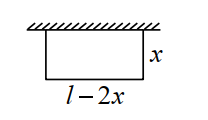
\includegraphics{D:/sslchi.github.io/calculus/HW_chap4b.png}
%		\caption{}
%	\end{figure}

\begin{solution}如图, 设靠河的篱笆长为 $x$, 则矩形场地的面积为
$$S = x(l - 2x),$$则
$$S' = l - 4 x$$, 得唯一驻点 $\displaystyle x = \frac{l}{4}$.
显然存在最大面积, 所以
$$S_{\max} = S\left( \frac{l}{4} \right) = \frac{l^{2}}{8}.$$
\end{solution}

\kpoint{函数最值的应用}

\end{problem}        

  
\begin{problem} 要做一个圆锥形漏斗, 其母线长 20 cm, 要使其体积最大, 问其高应为多少?

\begin{solution} 设圆锥形漏斗的高为 $H$cm, 则圆锥底面半径为
$$R = \sqrt{400 - H^{2}}$$
漏斗的体积为
$$V = \frac{\pi}{3}\left( 400 - H^{2} \right)H,\ 0 < H < 20,$$

又因为
$$V' = \frac{\pi}{3}\left( 400 - 3H^{2} \right),$$

所以体积函数 $V$ 在$(0, 20)$内有唯一驻点
$$H = \frac{20\sqrt{3}}{3},$$

又因为
$$V'' = - 2\pi H < 0,$$

因此唯一驻点 $\displaystyle H = \frac{20\sqrt{3}}{3}$ 也是极大值点, 由实际问题可知,
此时漏斗体积最大.
\end{solution}
\kpoint{函数最值的应用}

\end{problem}           

\begin{problem} 设有一块边长为 $a$ 的正方形铁皮, 从四个角截去同样的小方块,
做成一个无盖的方盒子, 问小方块的边长为多少才使盒子的容积最大?

\begin{solution} 设小方块的边长为 $x$, 则盒子的容积为
$$V = x\left( a - 2x \right)^{2} = a^{2}x + 4x^{3} - 4ax^{2},\quad 0 < x < \frac{a}{2},$$

其导数为
$$V' = a^{2} + 12x^{2} - 8ax$$

唯一驻点 $\displaystyle x = \frac{a}{6}$. 又
$$\left. \ V'' \right|_{x = \frac{a}{6}} = \left. \ \left( 24x - 8a \right) \right|_{x = \frac{a}{6}} = - 4a < 0,$$

即 $\displaystyle x = \frac{a}{6}$ 为极大值点, 也是最大值, 所以小方块边长为
$\displaystyle \frac{a}{6}$ 时, 盒子的容积最大.
\end{solution}
\kpoint{函数最值的应用}

\end{problem}           

\begin{problem} 设某产品的销售量 $Q$ 与价格 $P$ 之间有关系式为
$\displaystyle Q = \frac{1 - P}{P}$

(1) 求需求弹性 ;

(2) 售价为 $0.5$ 时的需求弹性. 并给出经济解释.

\begin{solution}(1)
$$\eta = - Q'\left( P \right)\frac{P}{Q\left( P \right)} = \frac{1}{P^{2}}\frac{P}{\frac{1 - P}{P}} = \frac{1}{1 - P}$$

(2)
$$\eta\left( 0.5 \right) = \left. \ \frac{1}{1 - P} \right|_{P = 0.5} = 2$$

其经济意义为: 在售价为 $0.5$ 时的水平上, 若价格上涨 $1\%$,
需求量下降 $2\%.$
\end{solution}
\kpoint{弹性(应该放在第三章)}

\end{problem}           

\begin{problem} 某厂生产某种商品, 其年销售量为 $100$ 万件,
每批生产需增加准备费1000元, 而每件的库存费为0.05元. 如果年销售是均匀的,
且上批销售完后, 立即再生产下一批(此时商品库存量为批量的一半),
问分几批生产, 能使生产准备费及库存费之和最小?

\begin{solution} 设每批生产 $x$ 件, 则有
$$y = 1000 \times \frac{1000000}{x} - \frac{x}{2} \times 0.05,$$
其导数为:
$$y' = \frac{10^{9}}{x^{2}} - 0.025$$

令 $y' = 0$, 得 $x = 200000$ (件)(舍去负根).
$$y'' = \frac{2 \times 10^{9}}{x^{3}},\ y''\left( 200000 \right) > 0,$$

即批量 $200000$(件), 批次为 $5$ 时总费用最小.
\end{solution}
\kpoint{函数最值的应用}

\end{problem}           

\begin{problem} 某商品的价格 $P$ 与需求量 $Q$ 的关系为 $\displaystyle P = 10 - \frac{Q}{5}$,

(1) 求需求量为 $20$ 及 $30$ 时的总收益 $R$、平均收益
$\overline{R}$ 及边际收益 $R'$;

(2) $Q$ 为多少时总收益最大?

\begin{solution}
由条件知
$$R = R\left( Q \right) = QP\left( Q \right) = 10Q - \frac{Q^{2}}{5}$$
$$\overline{R}\left( Q \right) = P\left( Q \right)$$
$$R'\left( Q \right) = 10 - \frac{2Q}{5}$$

(1)由条件知:
$$R\left( 20 \right) = 120,R\left( 30 \right) = 120,\overline{R}\left( 20 \right) = 6,$$
$$\overline{R}\left( 30 \right) = 4,R'\left( 20 \right) = 2,R'\left( 30 \right) = - 2.$$

(2) 令 $R'\left( Q \right) = 0$, 得 $Q = 25$, 又
$$R''\left( Q \right) = - \frac{2}{5} < 0,$$ 所以 $Q = 25$
时总收益最大.
\end{solution}
\kpoint{函数最值的应用}

\end{problem}           

\begin{problem} 设 $f\left( x \right) = x^{3} + ax^{2} + bx$ 在 $x = 1$ 处有极值
$- 2$, 试确定系数 $a,\ b,$ 并求出 $y = f\left( x \right)$
的所有极值点及拐点.

\begin{solution} 由题意知
$$f'\left( x \right) = 3x^{2} + 2ax + b$$

由于 $f\left( x \right)$ 在点 $x = 1$ 有极值 $- 2$, 所以
$$f\left( 1 \right) = 1 + a + b = - 2,\ f'\left( 1 \right) = 3 + 2a + b = 0 \Rightarrow a = 0,b = - 3,$$

因此
$$f\left( x \right) = x^{3} - 3x,f'\left( x \right) = 3x^{2} - 3,f''\left( x \right) = 6x.$$

所以极值点为 $x = 1$ 和 $x = - 1,$ 拐点为 $(0, 0).$
\end{solution}
\kpoint{函数极值的第二充分条件}

\end{problem}           

\begin{problem} 在半径为 $R$ 的球内, 求体积最大的内接圆柱体的高.

\begin{solution} 设内接圆柱体的高为 $h$ , 则圆柱体的底面半径
$$r = \sqrt{R^{2} - \left( \frac{h}{2} \right)^{2}},$$

其体积为
$$V = \pi h\left( R^{2} - \frac{h^{2}}{4} \right),\quad 0 < h < 2R,$$

其导函数为
$$V' = \pi\left( R^{2} - \frac{3}{4}h^{2} \right)$$

故其有唯一驻点
$$h = \frac{2\sqrt{3}}{3}R,$$

又因为
$$V'' = - \frac{3}{2}\pi h < 0,$$

故 $\displaystyle h = \frac{2\sqrt{3}}{3}R$ 时, 圆柱体体积最大.
\end{solution}
\kpoint{函数最值的应用}

\end{problem}           

\begin{problem} 由三块同一宽度的板做成一个梯形的排水槽(无上盖), 问侧面与底的倾角
$\alpha$ 为多大时, 才使水槽的横断面积最大?

\begin{solution} 设板宽为 $a$, 侧面与底面的倾角为 $\alpha$ 则横断面面积为
$$S = \frac{1}{2}\left( 2a + 2a\cos\alpha \right)a\sin\alpha = a^{2}\left( 1 + \cos\alpha \right)\sin\alpha,\ \  0 < \alpha < \frac{\pi}{2}.$$

其导数为
$$S' = a^{2}\left( 2\cos^{2}\alpha + \cos\alpha - 1 \right)$$

该函数的唯一驻点 $\alpha = \frac{\pi}{3}$.

又因为
$$S'' = - a^{2}\left( 2\sin 2\alpha + \sin\alpha \right),\left. \ \quad S'' \right|_{\alpha = \frac{\pi}{3}} = - \frac{3\sqrt{3}}{2}a^{2} < 0$$

所以当 $\displaystyle \alpha = \frac{\pi}{3}$ 时, 横断面面积最大.
\end{solution}
\kpoint{函数最值的应用}

\end{problem}           


\begin{problem} 将半径为 $r$ 的圆铁片, 剪去一个扇形, 问其中心角 $\alpha$
为多大时, 才能使余下部分围成的圆锥形容器的容积最大?

\begin{solution} 设圆雉形容器半径为 $R$, 高为 $h$, 容积为 $V$, 则
$$R^{2} + h^{2} = r^{2},V = \frac{1}{3}\pi R^{2}h = \frac{\pi}{3}\left( r^{2} - h^{2} \right)h$$

令
$$\frac{\text{d}V}{\text{d}h} = \frac{\pi}{3}\left( r^{2} - 3h^{2} \right) = 0,$$
求得的唯一驻点为 $$h = \frac{r}{\sqrt{3}},$$ 此时
$\displaystyle R = \frac{\sqrt{2}}{\sqrt{3}}\text{r.}$ 依问题的实际意义, $V$
存在最大值.故 $\displaystyle R = \frac{\sqrt{2}}{\sqrt{3}}r$ 为所求 , 但
$$2\pi R = \left( 2\pi - \alpha \right)r,$$ 解得
$$\alpha = \left( 1 - \frac{\sqrt{6}}{3} \right) \cdot 2.$$ 即
$$\alpha = 1 - \frac{\sqrt{6}}{3} \cdot 2$$ 时所求容积最大.
\end{solution}
\kpoint{函数最值的应用}

\end{problem}

\makepart{证明题}



\begin{problem} 设 $f\left( x \right)$ 在 $\left\lbrack 1,\e \right\rbrack$
上连续, 在 $(1,\e)$ 内可导, 且
$f\left( 1 \right) = 0,f\left( \e \right) = 1,$ 证明方程
$xf'\left( x \right) = 1$ 在 $\left( 1,\e \right)$ 内至少有一实根.

\begin{solution}
证明: 令 $F\left( x \right) = f\left( x \right) - \ln x,$ 则
$F\left( x \right)$ 在 $\left\lbrack 1,\e \right\rbrack$ 上连续, 在
$(1,\e)$ 内可导. {因}
$f\left( 1 \right) = 0,f\left( \e \right) = 1,$ {则}
$F\left( 1 \right) = F\left( \e \right) = 0,$ {即}
$F\left( x \right)$ {在} $\left\lbrack 1,\e \right\rbrack$
{上满足罗尔定理的条件, 则至少存在}
$\xi \in \left( 1,\e \right)${, 使} $F'\left( \xi \right) = 0,$
而
$$F'\left( x \right) = f'\left( x \right) - \frac{1}{x},$$
即
$$f'\left( \xi \right) - \frac{1}{\xi} = 0,\quad\xi \in \left( 1,\e \right)$$
即
$$\xi f'\left( \xi \right) = 1.$$
故 $xf'\left( x \right) = 1$ 在 $(1,\e)$ 内至少有一个实根.

\end{solution}

\kpoint{罗尔定理}


\end{problem}           


\begin{problem} 设 $f\left( x \right)$ 在 $\left\lbrack a,b \right\rbrack$
上可导, 证明存在 $\xi \in \left( a,b \right),$ 使
$$\frac{1}{b - a}\left| \begin{matrix}
b^{3} & a^{3} \\
f\left( a \right) & f\left( b \right) \\
\end{matrix} \right| = \xi^{2}\left\lbrack 3 f\left( \xi \right) + \xi f'\left( \xi \right) \right\rbrack.$$

\begin{solution}
	证明: 令 $F\left( x \right) = x^{3}f\left( x \right),$ 则
$F\left( x \right)$ 在 $\left\lbrack a,b \right\rbrack$ 上可导,
利用拉格朗日中值定理, 则至少存在 $\xi \in \left( a,b \right),$ 使
$$F\left( b \right) - F\left( a \right) = F'\left( \xi \right)\left( b - a \right),$$
即
$$b^{3}f\left( b \right) - a^{3}f\left( a \right) = \left\lbrack 3\xi^{2}f\left( \xi \right) + \xi^{3}f'\left( \xi \right) \right\rbrack\left( b - a \right),$$
即
$$\frac{1}{b - a}\left| \begin{matrix}
b^{3} & a^{3} \\
f\left( a \right) & f\left( b \right) \\
\end{matrix} \right| = \xi^{2}\left\lbrack 3 f\left( \xi \right) + \xi f'\left( \xi \right) \right\rbrack.$$
\end{solution}

\kpoint{拉格朗日中值定理}
\end{problem} 

\begin{problem}
设 $f\left( x \right)$ {在}
$\left\lbrack 1,2 \right\rbrack$ {上连续, 在} $(1,\ 2)$
{内可导, 且} $f\left( 2 \right) = 0,$ {证明至少存在一点}
$\xi \in \left( 1,2 \right),$ {使}
$$f'\left( \xi \right) = - \frac{f\left( \xi \right)}{\xi\ln\left( \xi \right)}.$$

\begin{solution}
{证明: 令} $F\left( x \right) = f\left( x \right)\ln x${,
	则} $F\left( x \right)$ {在} $\lbrack 1,\ 2\rbrack$
{上连续, 在} $(1,\ 2)$ {内可导, 且}
$$F\left( 1 \right) = f\left( 1 \right)\ln 1 = 0,\quad F\left( 2 \right) = f\left( 2 \right)\ln 2 = 0.$$

{即} $F\left( x \right)$ {在} $\lbrack 1,2\rbrack$
{上满足罗尔定理的条件, 则至少存在}
$\xi \in \left( 1, 2 \right)$ {使}
$F'\left( \xi \right) = 0,$ {而}
$$F'\left( x \right) = f'\left( x \right)\ln x + f\left( x \right) \cdot \frac{1}{x}$$
{即有}
$$f'\left( \xi \right) = - \frac{f\left( \xi \right)}{\xi\ln\left( \xi \right)}.$$

\end{solution}
\kpoint{罗尔定理}

\end{problem}           

\begin{problem} 设 $b > a > 0,$ {证明 :}
$\displaystyle \ln\frac{b}{a} > \frac{2\left( b - a \right)}{a + b}.$

\begin{solution}
证明: 令
$f\left( x \right) = \left( a + x \right)\left( \ln x - \ln a \right) - 2\left( x - a \right),$则
$$f\left( a \right) = 0,f'\left( x \right) = \ln x–\ln a + \left( a + x \right)\frac{1}{x} - 2,$$
{即}
$$f'\left( x \right) = \ln x - \ln a + \frac{a}{x} - 1$$
{故} $f'\left( a \right) = 0.$ {又因为}
$$f''\left( x \right) = \frac{1}{x} - \frac{a}{x^{2}} = \frac{x - a}{x^{2}} > 0\quad\left( x > a \right),$$
{所以} $f''\left( x \right)$ {单调递增,}
$f'\left( x \right) > f\left( a \right) = 0,$ {所以函数}
$f\left( x \right)$ {单调递增, 于是当} $x > a$ {时}
$f\left( x \right) > f\left( a \right) = 0,$ {令}
$x = b${, 则} $f\left( b \right) > f\left( a \right) = 0,$
{即}
$$\left( a + b \right)\left( \ln b - \ln a \right) - 2\left( b - a \right) > 0,$$
{亦即}
$$\ln\frac{b}{a} > \frac{2\left( b - a \right)}{a + b}.$$
\end{solution}
\kpoint{ 函数单调性的判别法}

\end{problem}           

\begin{problem} 证明当 $x \neq 0$ {时, 有不等式} $\e^{x} > 1 + x.$

\begin{solution}
证明:令 $$f\left( x \right) = \e^{x} - x - 1,$$
它在
$\left( - \infty, + \infty \right)$ 连续.易知
$$f'\left( x \right) = \e^{x} - 1,\ f''\left( x \right) = \e^{x} > 0.\
f'\left( 0 \right) = 0,f''\left( 0 \right) > 0,$$
所以
$f\left( 0 \right)$ {是} $f\left( x \right)$
{的极小值也是最小值, 当} $x \neq 0$ {时, 得}
$$f\left( x \right) > f\left( 0 \right),$$ {故} $x \neq 0$
{时,}
$$\e^{x} > 1 + x.$$
\end{solution}

\kpoint{函数极值的第二充分条件}
\end{problem} 